\biohead{Eric Geoffrey West Hancox}{Eric_Geoffrey_West_Hancox}{Geoff in the 1930s\citeref{}}

%\section{Eric Geoffrey West Hancox}\label{Eric_Geoffrey_West_Hancox}
%\begin{center}
%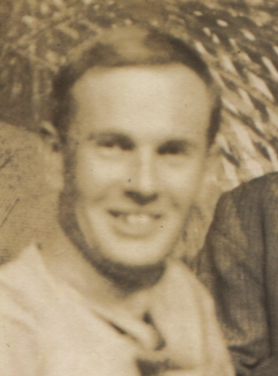
\includegraphics[width=0.8\linewidth]{photos/Eric_Geoffrey_West_Hancox}
%\end{center}

Eric Geoffrey West ``Geoff'' Hancox (July 1911 -- 10 August 1937). Arrived in New York on the Scythia, 11 September 1934 (listed as a student)(S4). The following year he came into the US from Canada, to Babb, Montana, and is listed as a student at both the University of California and Tuscon, Arizona (S5); he was a PhD student in Geology. He died in 1937 in a mining accident in Burma.

Probate announcement:
\begin{quotation}
Probate: Hancox Eric Geoffrey of Morant, Herbert Road, New Milton, Hampshire died 10 August 1937 at Mawchi Mines Burma India. Administration Winchester 26 November to Richard James Hancox retired bank inspecor. Effects (pounds)734.19s.9d.
\end{quotation}


\begin{quotation}
Recognition Given U Of A By British TUCSON May recognition of the strength of the department of geology at the University of Arizona and of the wealth of field research opportunity in the state has come through the announcement that a Common- wealth Fund Fellowship has been awarded to an English student for specific graduate study at the University of Arizona. President Homer LeRoy Shants of the University indicated today that the selection of the University of Arizona for one of these school places its department on an equal plane with the great centers of study in that field. The fellowship has been awarded to Eric Geoffrey Hancox a graduate of the University of Liverpool and of the Imperial College of Science London University.
\end{quotation}
